\documentclass[twoside]{book}

% Packages required by doxygen
\usepackage{fixltx2e}
\usepackage{calc}
\usepackage{doxygen}
\usepackage[export]{adjustbox} % also loads graphicx
\usepackage{graphicx}
\usepackage[utf8]{inputenc}
\usepackage{makeidx}
\usepackage{multicol}
\usepackage{multirow}
\PassOptionsToPackage{warn}{textcomp}
\usepackage{textcomp}
\usepackage[nointegrals]{wasysym}
\usepackage[table]{xcolor}

% Font selection
\usepackage[T1]{fontenc}
\usepackage[scaled=.90]{helvet}
\usepackage{courier}
\usepackage{amssymb}
\usepackage{sectsty}
\renewcommand{\familydefault}{\sfdefault}
\allsectionsfont{%
  \fontseries{bc}\selectfont%
  \color{darkgray}%
}
\renewcommand{\DoxyLabelFont}{%
  \fontseries{bc}\selectfont%
  \color{darkgray}%
}
\newcommand{\+}{\discretionary{\mbox{\scriptsize$\hookleftarrow$}}{}{}}

% Page & text layout
\usepackage{geometry}
\geometry{%
  a4paper,%
  top=2.5cm,%
  bottom=2.5cm,%
  left=2.5cm,%
  right=2.5cm%
}
\tolerance=750
\hfuzz=15pt
\hbadness=750
\setlength{\emergencystretch}{15pt}
\setlength{\parindent}{0cm}
\setlength{\parskip}{3ex plus 2ex minus 2ex}
\makeatletter
\renewcommand{\paragraph}{%
  \@startsection{paragraph}{4}{0ex}{-1.0ex}{1.0ex}{%
    \normalfont\normalsize\bfseries\SS@parafont%
  }%
}
\renewcommand{\subparagraph}{%
  \@startsection{subparagraph}{5}{0ex}{-1.0ex}{1.0ex}{%
    \normalfont\normalsize\bfseries\SS@subparafont%
  }%
}
\makeatother

% Headers & footers
\usepackage{fancyhdr}
\pagestyle{fancyplain}
\fancyhead[LE]{\fancyplain{}{\bfseries\thepage}}
\fancyhead[CE]{\fancyplain{}{}}
\fancyhead[RE]{\fancyplain{}{\bfseries\leftmark}}
\fancyhead[LO]{\fancyplain{}{\bfseries\rightmark}}
\fancyhead[CO]{\fancyplain{}{}}
\fancyhead[RO]{\fancyplain{}{\bfseries\thepage}}
\fancyfoot[LE]{\fancyplain{}{}}
\fancyfoot[CE]{\fancyplain{}{}}
\fancyfoot[RE]{\fancyplain{}{\bfseries\scriptsize Generated by Doxygen }}
\fancyfoot[LO]{\fancyplain{}{\bfseries\scriptsize Generated by Doxygen }}
\fancyfoot[CO]{\fancyplain{}{}}
\fancyfoot[RO]{\fancyplain{}{}}
\renewcommand{\footrulewidth}{0.4pt}
\renewcommand{\chaptermark}[1]{%
  \markboth{#1}{}%
}
\renewcommand{\sectionmark}[1]{%
  \markright{\thesection\ #1}%
}

% Indices & bibliography
\usepackage{natbib}
\usepackage[titles]{tocloft}
\setcounter{tocdepth}{3}
\setcounter{secnumdepth}{5}
\makeindex

% Hyperlinks (required, but should be loaded last)
\usepackage{ifpdf}
\ifpdf
  \usepackage[pdftex,pagebackref=true]{hyperref}
\else
  \usepackage[ps2pdf,pagebackref=true]{hyperref}
\fi
\hypersetup{%
  colorlinks=true,%
  linkcolor=blue,%
  citecolor=blue,%
  unicode%
}

% Custom commands
\newcommand{\clearemptydoublepage}{%
  \newpage{\pagestyle{empty}\cleardoublepage}%
}

\usepackage{caption}
\captionsetup{labelsep=space,justification=centering,font={bf},singlelinecheck=off,skip=4pt,position=top}

%===== C O N T E N T S =====

\begin{document}

% Titlepage & ToC
\hypersetup{pageanchor=false,
             bookmarksnumbered=true,
             pdfencoding=unicode
            }
\pagenumbering{alph}
\begin{titlepage}
\vspace*{7cm}
\begin{center}%
{\Large My Project }\\
\vspace*{1cm}
{\large Generated by Doxygen 1.8.13}\\
\end{center}
\end{titlepage}
\clearemptydoublepage
\pagenumbering{roman}
\tableofcontents
\clearemptydoublepage
\pagenumbering{arabic}
\hypersetup{pageanchor=true}

%--- Begin generated contents ---
\chapter{Main Page}
\label{index}\hypertarget{index}{}This is the main file of the program. This will be used to launch the interface to select files and other things. Refer to class list for detailed description of other classes. 
\chapter{Class Index}
\section{Class List}
Here are the classes, structs, unions and interfaces with brief descriptions\+:\begin{DoxyCompactList}
\item\contentsline{section}{\hyperlink{classEdgeLoop}{Edge\+Loop} }{\pageref{classEdgeLoop}}{}
\item\contentsline{section}{\hyperlink{classpartialOrder}{partial\+Order} }{\pageref{classpartialOrder}}{}
\item\contentsline{section}{\hyperlink{classVertice}{Vertice} }{\pageref{classVertice}}{}
\item\contentsline{section}{\hyperlink{classWireFrame}{Wire\+Frame} }{\pageref{classWireFrame}}{}
\end{DoxyCompactList}

\chapter{File Index}
\section{File List}
Here is a list of all files with brief descriptions\+:\begin{DoxyCompactList}
\item\contentsline{section}{/home/ankurshaswat/\+My\+Files/\+Repos/\+C\+O\+P290/\+Project1/\+Code/include/module1/\hyperlink{Display_8h}{Display.\+h} }{\pageref{Display_8h}}{}
\item\contentsline{section}{/home/ankurshaswat/\+My\+Files/\+Repos/\+C\+O\+P290/\+Project1/\+Code/include/module1/\hyperlink{Edge_8h}{Edge.\+h} }{\pageref{Edge_8h}}{}
\item\contentsline{section}{/home/ankurshaswat/\+My\+Files/\+Repos/\+C\+O\+P290/\+Project1/\+Code/include/module1/\hyperlink{EdgeLoop_8h}{Edge\+Loop.\+h} }{\pageref{EdgeLoop_8h}}{}
\item\contentsline{section}{/home/ankurshaswat/\+My\+Files/\+Repos/\+C\+O\+P290/\+Project1/\+Code/include/module1/\hyperlink{Face_8h}{Face.\+h} }{\pageref{Face_8h}}{}
\item\contentsline{section}{/home/ankurshaswat/\+My\+Files/\+Repos/\+C\+O\+P290/\+Project1/\+Code/include/module1/\hyperlink{Fig2D_8h}{Fig2\+D.\+h} }{\pageref{Fig2D_8h}}{}
\item\contentsline{section}{/home/ankurshaswat/\+My\+Files/\+Repos/\+C\+O\+P290/\+Project1/\+Code/include/module1/\hyperlink{Fig3D_8h}{Fig3\+D.\+h} }{\pageref{Fig3D_8h}}{}
\item\contentsline{section}{/home/ankurshaswat/\+My\+Files/\+Repos/\+C\+O\+P290/\+Project1/\+Code/include/module1/\hyperlink{Vertice_8h}{Vertice.\+h} }{\pageref{Vertice_8h}}{}
\item\contentsline{section}{/home/ankurshaswat/\+My\+Files/\+Repos/\+C\+O\+P290/\+Project1/\+Code/include/module1/\hyperlink{Wireframe_8h}{Wireframe.\+h} }{\pageref{Wireframe_8h}}{}
\item\contentsline{section}{/home/ankurshaswat/\+My\+Files/\+Repos/\+C\+O\+P290/\+Project1/\+Code/src/\hyperlink{program_8cpp}{program.\+cpp} \\*Main file documentation }{\pageref{program_8cpp}}{}
\item\contentsline{section}{/home/ankurshaswat/\+My\+Files/\+Repos/\+C\+O\+P290/\+Project1/\+Code/src/module1/\hyperlink{Fig3D_8cpp}{Fig3\+D.\+cpp} }{\pageref{Fig3D_8cpp}}{}
\end{DoxyCompactList}

\chapter{Class Documentation}
\hypertarget{classEdge}{}\section{Edge Class Reference}
\label{classEdge}\index{Edge@{Edge}}


{\ttfamily \#include $<$Edge.\+h$>$}



The documentation for this class was generated from the following file\+:\begin{DoxyCompactItemize}
\item 
/home/ankurshaswat/\+My\+Files/\+Repos/\+C\+O\+P290/\+Project1/\+Code/include/module1/\hyperlink{Edge_8h}{Edge.\+h}\end{DoxyCompactItemize}

\hypertarget{classEdgeLoop}{}\section{Edge\+Loop Class Reference}
\label{classEdgeLoop}\index{Edge\+Loop@{Edge\+Loop}}


{\ttfamily \#include $<$complex\+Components.\+h$>$}

\subsection*{Public Member Functions}
\begin{DoxyCompactItemize}
\item 
bool \hyperlink{classEdgeLoop_acae6f647805e3f043325f047208556c8}{is\+Contained} (\hyperlink{classEdgeLoop}{Edge\+Loop} a)
\end{DoxyCompactItemize}
\subsection*{Public Attributes}
\begin{DoxyCompactItemize}
\item 
vector$<$ \hyperlink{structVertice}{Vertice} $>$ \hyperlink{classEdgeLoop_a781d9dd73f8b69c7b0075d4297f6b277}{vertices}
\end{DoxyCompactItemize}


\subsection{Detailed Description}
Some high level components used as intermediates in our algorithms a planar closed loop of edges (connected end-\/to-\/end) 

\subsection{Member Function Documentation}
\mbox{\Hypertarget{classEdgeLoop_acae6f647805e3f043325f047208556c8}\label{classEdgeLoop_acae6f647805e3f043325f047208556c8}} 
\index{Edge\+Loop@{Edge\+Loop}!is\+Contained@{is\+Contained}}
\index{is\+Contained@{is\+Contained}!Edge\+Loop@{Edge\+Loop}}
\subsubsection{\texorpdfstring{is\+Contained()}{isContained()}}
{\footnotesize\ttfamily bool Edge\+Loop\+::is\+Contained (\begin{DoxyParamCaption}\item[{\hyperlink{classEdgeLoop}{Edge\+Loop}}]{a }\end{DoxyParamCaption})}

Function to check whether an edge\+Loop is completely contained in another 

\subsection{Member Data Documentation}
\mbox{\Hypertarget{classEdgeLoop_a781d9dd73f8b69c7b0075d4297f6b277}\label{classEdgeLoop_a781d9dd73f8b69c7b0075d4297f6b277}} 
\index{Edge\+Loop@{Edge\+Loop}!vertices@{vertices}}
\index{vertices@{vertices}!Edge\+Loop@{Edge\+Loop}}
\subsubsection{\texorpdfstring{vertices}{vertices}}
{\footnotesize\ttfamily vector$<$\hyperlink{structVertice}{Vertice}$>$ Edge\+Loop\+::vertices}



The documentation for this class was generated from the following file\+:\begin{DoxyCompactItemize}
\item 
/home/ankurshaswat/\+My\+Files/\+Repos/\+C\+O\+P290-\/master/\+E\+D\+\_\+\+Project/include/\hyperlink{complexComponents_8h}{complex\+Components.\+h}\end{DoxyCompactItemize}

\hypertarget{classFace}{}\section{Face Class Reference}
\label{classFace}\index{Face@{Face}}


{\ttfamily \#include $<$Face.\+h$>$}

\subsection*{Public Member Functions}
\begin{DoxyCompactItemize}
\item 
\hyperlink{classEdge}{Edge} $\ast$ \hyperlink{classFace_a5973ddd3395e60aeadc76f24d1bcc860}{get\+Edges} ()
\item 
vector$<$ vector$<$ \hyperlink{classEdge}{Edge} $>$ $>$ \hyperlink{classFace_a3676c176d0ad0b518a74409372aa94da}{planar\+Partitions} ()
\end{DoxyCompactItemize}


\subsection{Member Function Documentation}
\mbox{\Hypertarget{classFace_a5973ddd3395e60aeadc76f24d1bcc860}\label{classFace_a5973ddd3395e60aeadc76f24d1bcc860}} 
\index{Face@{Face}!get\+Edges@{get\+Edges}}
\index{get\+Edges@{get\+Edges}!Face@{Face}}
\subsubsection{\texorpdfstring{get\+Edges()}{getEdges()}}
{\footnotesize\ttfamily \hyperlink{classEdge}{Edge}$\ast$ Face\+::get\+Edges (\begin{DoxyParamCaption}{ }\end{DoxyParamCaption})}

\mbox{\Hypertarget{classFace_a3676c176d0ad0b518a74409372aa94da}\label{classFace_a3676c176d0ad0b518a74409372aa94da}} 
\index{Face@{Face}!planar\+Partitions@{planar\+Partitions}}
\index{planar\+Partitions@{planar\+Partitions}!Face@{Face}}
\subsubsection{\texorpdfstring{planar\+Partitions()}{planarPartitions()}}
{\footnotesize\ttfamily vector$<$ vector$<$\hyperlink{classEdge}{Edge}$>$ $>$ Face\+::planar\+Partitions (\begin{DoxyParamCaption}{ }\end{DoxyParamCaption})}



The documentation for this class was generated from the following files\+:\begin{DoxyCompactItemize}
\item 
/home/ankurshaswat/\+My\+Files/\+Repos/\+C\+O\+P290/\+Project1/\+Code/include/module1/\hyperlink{Face_8h}{Face.\+h}\item 
/home/ankurshaswat/\+My\+Files/\+Repos/\+C\+O\+P290/\+Project1/\+Code/include/module1/\hyperlink{Wireframe_8h}{Wireframe.\+h}\end{DoxyCompactItemize}

\hypertarget{classFig3D}{}\section{Fig3D Class Reference}
\label{classFig3D}\index{Fig3D@{Fig3D}}


{\ttfamily \#include $<$figures.\+h$>$}

\subsection*{Public Member Functions}
\begin{DoxyCompactItemize}
\item 
void \hyperlink{classFig3D_af1000067e4e230b41059896c8cacd4e1}{get\+Projections} (int plane, set$<$ \hyperlink{structEdge}{Edge} $>$ \&edge\+Set2D)
\item 
void \hyperlink{classFig3D_a4fbcfab626ef2fe938bc53dec4c0543a}{get\+Axes} (int plane, set$<$ \hyperlink{structEdge}{Edge} $>$ \&edge\+Set2D)
\item 
\hyperlink{classFig3D}{Fig3D} \hyperlink{classFig3D_a25a3607c2735064d0bc0081b271ea224}{get\+Transformation} (double Xrot, double Yrot, double Zrot, double Xoff, double Yoff, double Zoff)
\end{DoxyCompactItemize}
\subsection*{Public Attributes}
\begin{DoxyCompactItemize}
\item 
vector$<$ \hyperlink{structVertice}{Vertice} $>$ \hyperlink{classFig3D_a3d00aa545805c0c04563055cc183cbb9}{vertices}
\item 
vector$<$ vector$<$ unsigned int $>$ $>$ \hyperlink{classFig3D_abd9f97ce3404190fd202b12885d56fe3}{faces}
\end{DoxyCompactItemize}


\subsection{Detailed Description}
Defines classes for representing 2D views and 3D objects 

\subsection{Member Function Documentation}
\mbox{\Hypertarget{classFig3D_a4fbcfab626ef2fe938bc53dec4c0543a}\label{classFig3D_a4fbcfab626ef2fe938bc53dec4c0543a}} 
\index{Fig3D@{Fig3D}!get\+Axes@{get\+Axes}}
\index{get\+Axes@{get\+Axes}!Fig3D@{Fig3D}}
\subsubsection{\texorpdfstring{get\+Axes()}{getAxes()}}
{\footnotesize\ttfamily void Fig3\+D\+::get\+Axes (\begin{DoxyParamCaption}\item[{int}]{plane,  }\item[{set$<$ \hyperlink{structEdge}{Edge} $>$ \&}]{edge\+Set2D }\end{DoxyParamCaption})}

get XY, YZ , XZ and isometric projections of the 3D object get XY, YZ , XZ and isometric projections of the 3D object \mbox{\Hypertarget{classFig3D_af1000067e4e230b41059896c8cacd4e1}\label{classFig3D_af1000067e4e230b41059896c8cacd4e1}} 
\index{Fig3D@{Fig3D}!get\+Projections@{get\+Projections}}
\index{get\+Projections@{get\+Projections}!Fig3D@{Fig3D}}
\subsubsection{\texorpdfstring{get\+Projections()}{getProjections()}}
{\footnotesize\ttfamily void Fig3\+D\+::get\+Projections (\begin{DoxyParamCaption}\item[{int}]{plane,  }\item[{set$<$ \hyperlink{structEdge}{Edge} $>$ \&}]{edge\+Set2D }\end{DoxyParamCaption})}

get XY, YZ , XZ and isometric projections of the 3D object get XY, YZ , XZ and isometric projections of the 3D object \mbox{\Hypertarget{classFig3D_a25a3607c2735064d0bc0081b271ea224}\label{classFig3D_a25a3607c2735064d0bc0081b271ea224}} 
\index{Fig3D@{Fig3D}!get\+Transformation@{get\+Transformation}}
\index{get\+Transformation@{get\+Transformation}!Fig3D@{Fig3D}}
\subsubsection{\texorpdfstring{get\+Transformation()}{getTransformation()}}
{\footnotesize\ttfamily \hyperlink{classFig3D}{Fig3D} Fig3\+D\+::get\+Transformation (\begin{DoxyParamCaption}\item[{double}]{Xrot,  }\item[{double}]{Yrot,  }\item[{double}]{Zrot,  }\item[{double}]{Xoff,  }\item[{double}]{Yoff,  }\item[{double}]{Zoff }\end{DoxyParamCaption})}

get transformed 3D object get transformed 3D object 

\subsection{Member Data Documentation}
\mbox{\Hypertarget{classFig3D_abd9f97ce3404190fd202b12885d56fe3}\label{classFig3D_abd9f97ce3404190fd202b12885d56fe3}} 
\index{Fig3D@{Fig3D}!faces@{faces}}
\index{faces@{faces}!Fig3D@{Fig3D}}
\subsubsection{\texorpdfstring{faces}{faces}}
{\footnotesize\ttfamily vector$<$vector$<$unsigned int$>$ $>$ Fig3\+D\+::faces}

\mbox{\Hypertarget{classFig3D_a3d00aa545805c0c04563055cc183cbb9}\label{classFig3D_a3d00aa545805c0c04563055cc183cbb9}} 
\index{Fig3D@{Fig3D}!vertices@{vertices}}
\index{vertices@{vertices}!Fig3D@{Fig3D}}
\subsubsection{\texorpdfstring{vertices}{vertices}}
{\footnotesize\ttfamily vector$<$\hyperlink{structVertice}{Vertice}$>$ Fig3\+D\+::vertices}



The documentation for this class was generated from the following files\+:\begin{DoxyCompactItemize}
\item 
/home/ankurshaswat/\+My\+Files/\+Repos/\+C\+O\+P290/working\+\_\+3d\+\_\+to\+\_\+2d/include/module1/\hyperlink{figures_8h}{figures.\+h}\item 
/home/ankurshaswat/\+My\+Files/\+Repos/\+C\+O\+P290/working\+\_\+3d\+\_\+to\+\_\+2d/src/\hyperlink{figures_8cpp}{figures.\+cpp}\end{DoxyCompactItemize}

\hypertarget{classVertice}{}\section{Vertice Class Reference}
\label{classVertice}\index{Vertice@{Vertice}}


{\ttfamily \#include $<$Vertice.\+h$>$}



The documentation for this class was generated from the following file\+:\begin{DoxyCompactItemize}
\item 
/home/ankurshaswat/\+My\+Files/\+Repos/\+C\+O\+P290/\+Project1/\+Code/include/module1/\hyperlink{Vertice_8h}{Vertice.\+h}\end{DoxyCompactItemize}

\chapter{File Documentation}
\hypertarget{Display_8h}{}\section{/home/ankurshaswat/\+My\+Files/\+Repos/\+C\+O\+P290/\+Project1/\+Code/include/module1/\+Display.h File Reference}
\label{Display_8h}\index{/home/ankurshaswat/\+My\+Files/\+Repos/\+C\+O\+P290/\+Project1/\+Code/include/module1/\+Display.\+h@{/home/ankurshaswat/\+My\+Files/\+Repos/\+C\+O\+P290/\+Project1/\+Code/include/module1/\+Display.\+h}}

\hypertarget{Edge_8h}{}\section{/home/ankurshaswat/\+My\+Files/\+Repos/\+C\+O\+P290/\+Project1/\+Code/include/module1/\+Edge.h File Reference}
\label{Edge_8h}\index{/home/ankurshaswat/\+My\+Files/\+Repos/\+C\+O\+P290/\+Project1/\+Code/include/module1/\+Edge.\+h@{/home/ankurshaswat/\+My\+Files/\+Repos/\+C\+O\+P290/\+Project1/\+Code/include/module1/\+Edge.\+h}}
{\ttfamily \#include \char`\"{}Vertice.\+h\char`\"{}}\newline
Include dependency graph for Edge.\+h\+:\nopagebreak
\begin{figure}[H]
\begin{center}
\leavevmode
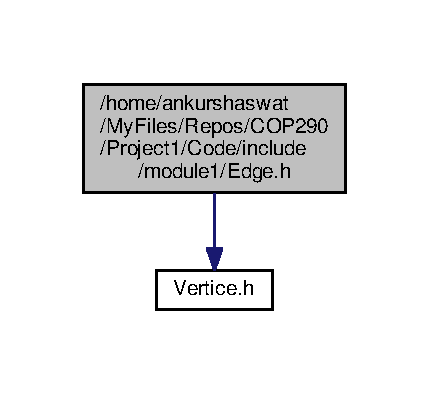
\includegraphics[width=206pt]{Edge_8h__incl}
\end{center}
\end{figure}
This graph shows which files directly or indirectly include this file\+:\nopagebreak
\begin{figure}[H]
\begin{center}
\leavevmode
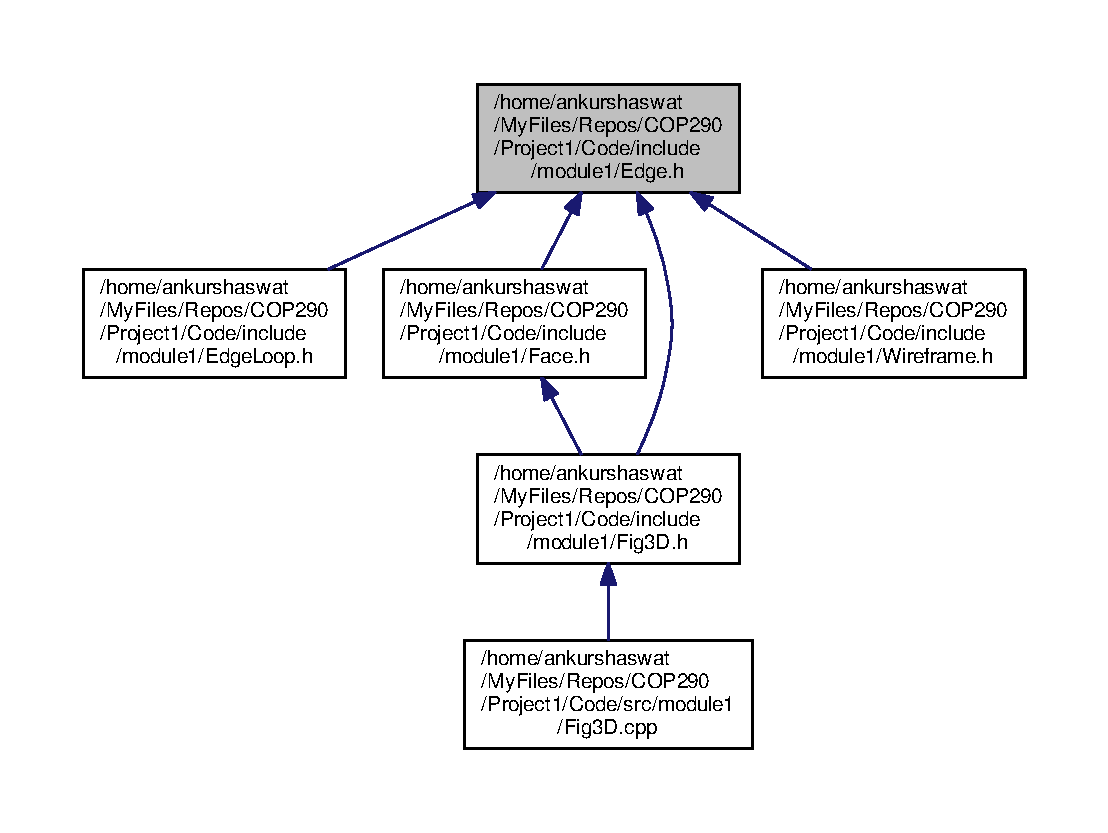
\includegraphics[width=350pt]{Edge_8h__dep__incl}
\end{center}
\end{figure}
\subsection*{Classes}
\begin{DoxyCompactItemize}
\item 
class \hyperlink{classEdge}{Edge}
\end{DoxyCompactItemize}

\hypertarget{EdgeLoop_8h}{}\section{/home/ankurshaswat/\+My\+Files/\+Repos/\+C\+O\+P290/\+Project1/\+Code/include/module1/\+Edge\+Loop.h File Reference}
\label{EdgeLoop_8h}\index{/home/ankurshaswat/\+My\+Files/\+Repos/\+C\+O\+P290/\+Project1/\+Code/include/module1/\+Edge\+Loop.\+h@{/home/ankurshaswat/\+My\+Files/\+Repos/\+C\+O\+P290/\+Project1/\+Code/include/module1/\+Edge\+Loop.\+h}}
{\ttfamily \#include \char`\"{}Edge.\+h\char`\"{}}\newline
Include dependency graph for Edge\+Loop.\+h\+:\nopagebreak
\begin{figure}[H]
\begin{center}
\leavevmode
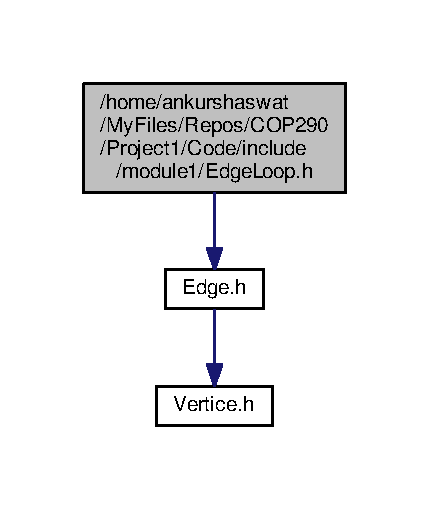
\includegraphics[width=206pt]{EdgeLoop_8h__incl}
\end{center}
\end{figure}
\subsection*{Classes}
\begin{DoxyCompactItemize}
\item 
class \hyperlink{classEdgeLoop}{Edge\+Loop}
\end{DoxyCompactItemize}

\hypertarget{Face_8h}{}\section{/home/ankurshaswat/\+My\+Files/\+Repos/\+C\+O\+P290/\+Project1/\+Code/include/module1/\+Face.h File Reference}
\label{Face_8h}\index{/home/ankurshaswat/\+My\+Files/\+Repos/\+C\+O\+P290/\+Project1/\+Code/include/module1/\+Face.\+h@{/home/ankurshaswat/\+My\+Files/\+Repos/\+C\+O\+P290/\+Project1/\+Code/include/module1/\+Face.\+h}}
{\ttfamily \#include \char`\"{}Edge.\+h\char`\"{}}\newline
{\ttfamily \#include \char`\"{}Vertice.\+h\char`\"{}}\newline
Include dependency graph for Face.\+h\+:
\nopagebreak
\begin{figure}[H]
\begin{center}
\leavevmode
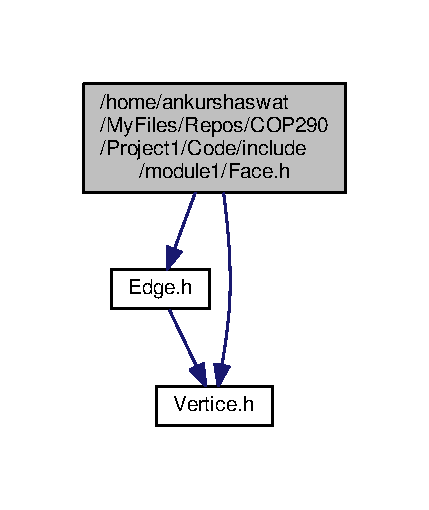
\includegraphics[width=206pt]{Face_8h__incl}
\end{center}
\end{figure}
This graph shows which files directly or indirectly include this file\+:
\nopagebreak
\begin{figure}[H]
\begin{center}
\leavevmode
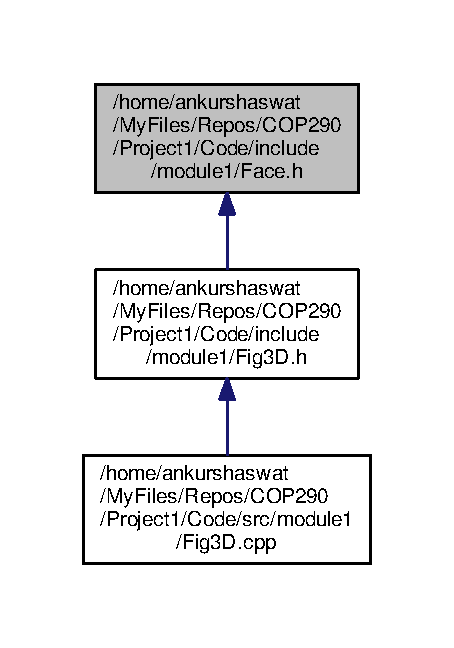
\includegraphics[width=218pt]{Face_8h__dep__incl}
\end{center}
\end{figure}
\subsection*{Classes}
\begin{DoxyCompactItemize}
\item 
class \hyperlink{classFace}{Face}
\end{DoxyCompactItemize}

\hypertarget{Fig2D_8h}{}\section{/home/ankurshaswat/\+My\+Files/\+Repos/\+C\+O\+P290/\+Project1/\+Code/include/module1/\+Fig2D.h File Reference}
\label{Fig2D_8h}\index{/home/ankurshaswat/\+My\+Files/\+Repos/\+C\+O\+P290/\+Project1/\+Code/include/module1/\+Fig2\+D.\+h@{/home/ankurshaswat/\+My\+Files/\+Repos/\+C\+O\+P290/\+Project1/\+Code/include/module1/\+Fig2\+D.\+h}}

\hypertarget{Fig3D_8h}{}\section{/home/ankurshaswat/\+My\+Files/\+Repos/\+C\+O\+P290/\+Project1/\+Code/include/module1/\+Fig3D.h File Reference}
\label{Fig3D_8h}\index{/home/ankurshaswat/\+My\+Files/\+Repos/\+C\+O\+P290/\+Project1/\+Code/include/module1/\+Fig3\+D.\+h@{/home/ankurshaswat/\+My\+Files/\+Repos/\+C\+O\+P290/\+Project1/\+Code/include/module1/\+Fig3\+D.\+h}}
{\ttfamily \#include \char`\"{}Face.\+h\char`\"{}}\newline
{\ttfamily \#include \char`\"{}Edge.\+h\char`\"{}}\newline
{\ttfamily \#include \char`\"{}Vertice.\+h\char`\"{}}\newline
Include dependency graph for Fig3\+D.\+h\+:\nopagebreak
\begin{figure}[H]
\begin{center}
\leavevmode
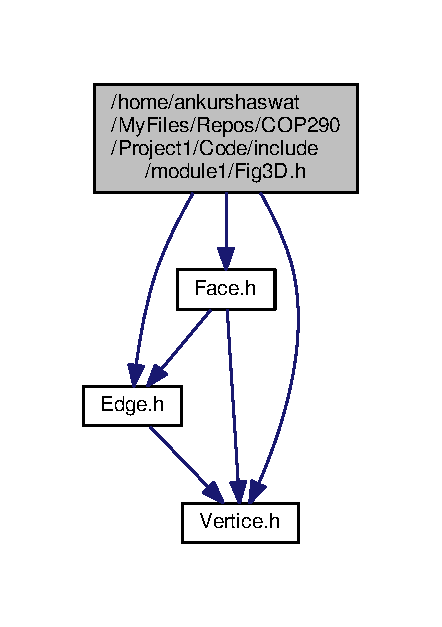
\includegraphics[width=212pt]{Fig3D_8h__incl}
\end{center}
\end{figure}
This graph shows which files directly or indirectly include this file\+:\nopagebreak
\begin{figure}[H]
\begin{center}
\leavevmode
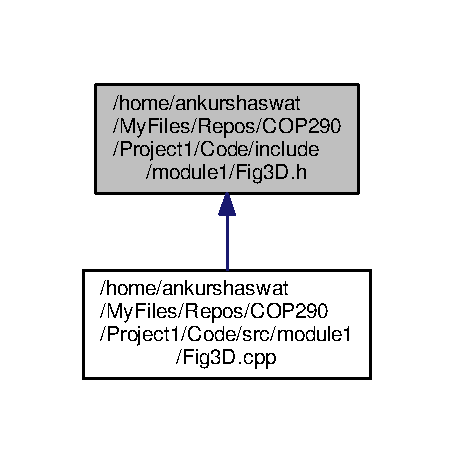
\includegraphics[width=218pt]{Fig3D_8h__dep__incl}
\end{center}
\end{figure}
\subsection*{Classes}
\begin{DoxyCompactItemize}
\item 
class \hyperlink{classFig3D}{Fig3D}
\end{DoxyCompactItemize}

\hypertarget{Vertice_8h}{}\section{/home/ankurshaswat/\+My\+Files/\+Repos/\+C\+O\+P290/\+Project1/\+Code/include/module1/\+Vertice.h File Reference}
\label{Vertice_8h}\index{/home/ankurshaswat/\+My\+Files/\+Repos/\+C\+O\+P290/\+Project1/\+Code/include/module1/\+Vertice.\+h@{/home/ankurshaswat/\+My\+Files/\+Repos/\+C\+O\+P290/\+Project1/\+Code/include/module1/\+Vertice.\+h}}
This graph shows which files directly or indirectly include this file\+:\nopagebreak
\begin{figure}[H]
\begin{center}
\leavevmode
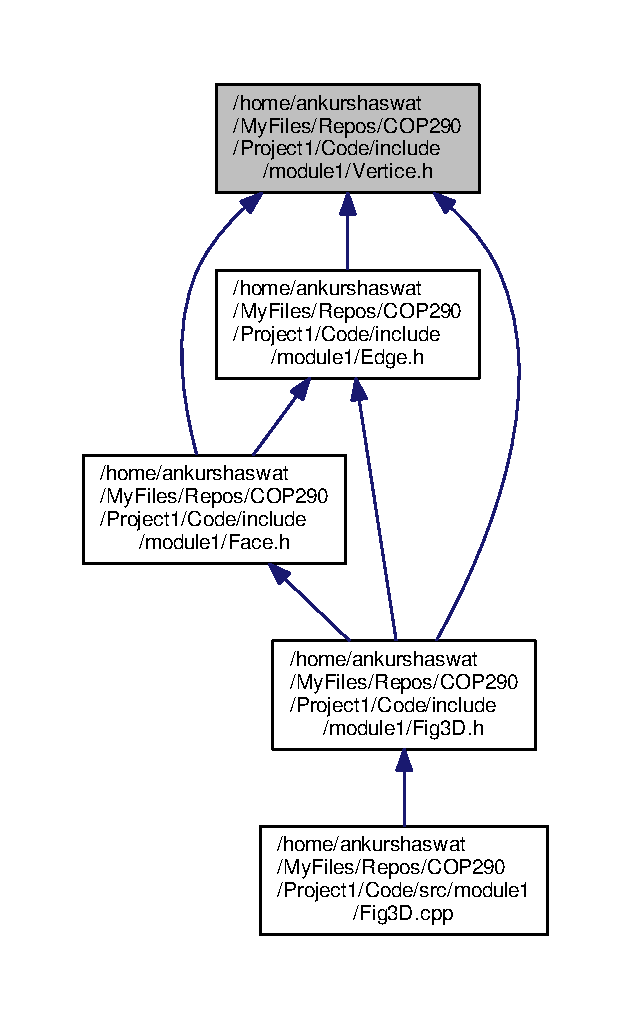
\includegraphics[width=350pt]{Vertice_8h__dep__incl}
\end{center}
\end{figure}
\subsection*{Classes}
\begin{DoxyCompactItemize}
\item 
class \hyperlink{classVertice}{Vertice}
\end{DoxyCompactItemize}

\hypertarget{Wireframe_8h}{}\section{/home/ankurshaswat/\+My\+Files/\+Repos/\+C\+O\+P290/\+Project1/\+Code/include/module1/\+Wireframe.h File Reference}
\label{Wireframe_8h}\index{/home/ankurshaswat/\+My\+Files/\+Repos/\+C\+O\+P290/\+Project1/\+Code/include/module1/\+Wireframe.\+h@{/home/ankurshaswat/\+My\+Files/\+Repos/\+C\+O\+P290/\+Project1/\+Code/include/module1/\+Wireframe.\+h}}

\hypertarget{Fig3D_8cpp}{}\section{/home/ankurshaswat/\+My\+Files/\+Repos/\+C\+O\+P290/\+Project1/\+Code/src/module1/\+Fig3D.cpp File Reference}
\label{Fig3D_8cpp}\index{/home/ankurshaswat/\+My\+Files/\+Repos/\+C\+O\+P290/\+Project1/\+Code/src/module1/\+Fig3\+D.\+cpp@{/home/ankurshaswat/\+My\+Files/\+Repos/\+C\+O\+P290/\+Project1/\+Code/src/module1/\+Fig3\+D.\+cpp}}
{\ttfamily \#include \char`\"{}module1/\+Fig3\+D.\+h\char`\"{}}\newline
Include dependency graph for Fig3\+D.\+cpp\+:
\nopagebreak
\begin{figure}[H]
\begin{center}
\leavevmode
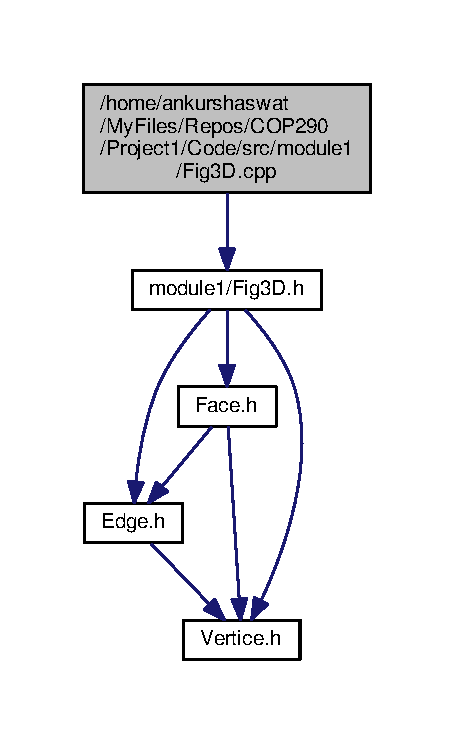
\includegraphics[width=218pt]{Fig3D_8cpp__incl}
\end{center}
\end{figure}

\hypertarget{program_8cpp}{}\section{/home/ankurshaswat/\+My\+Files/\+Repos/\+C\+O\+P290/\+Project1/\+Code/src/program.cpp File Reference}
\label{program_8cpp}\index{/home/ankurshaswat/\+My\+Files/\+Repos/\+C\+O\+P290/\+Project1/\+Code/src/program.\+cpp@{/home/ankurshaswat/\+My\+Files/\+Repos/\+C\+O\+P290/\+Project1/\+Code/src/program.\+cpp}}


Main file documentation.  


{\ttfamily \#include $<$iostream$>$}\newline
Include dependency graph for program.\+cpp\+:\nopagebreak
\begin{figure}[H]
\begin{center}
\leavevmode
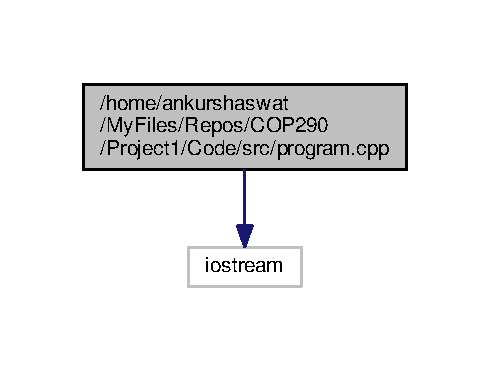
\includegraphics[width=235pt]{program_8cpp__incl}
\end{center}
\end{figure}
\subsection*{Functions}
\begin{DoxyCompactItemize}
\item 
int \hyperlink{program_8cpp_ae66f6b31b5ad750f1fe042a706a4e3d4}{main} ()
\end{DoxyCompactItemize}


\subsection{Detailed Description}
Main file documentation. 

\begin{DoxyAuthor}{Author}
Lastname\+:\+Firstname\+:\+A00123456\+:cscxxxxx 
\end{DoxyAuthor}
\begin{DoxyVersion}{Version}
Revision 1.\+0
\end{DoxyVersion}
Main File \begin{DoxyDate}{Date}
Monday, March 5, 2018 
\end{DoxyDate}


\subsection{Function Documentation}
\mbox{\Hypertarget{program_8cpp_ae66f6b31b5ad750f1fe042a706a4e3d4}\label{program_8cpp_ae66f6b31b5ad750f1fe042a706a4e3d4}} 
\index{program.\+cpp@{program.\+cpp}!main@{main}}
\index{main@{main}!program.\+cpp@{program.\+cpp}}
\subsubsection{\texorpdfstring{main()}{main()}}
{\footnotesize\ttfamily int main (\begin{DoxyParamCaption}{ }\end{DoxyParamCaption})}


%--- End generated contents ---

% Index
\backmatter
\newpage
\phantomsection
\clearemptydoublepage
\addcontentsline{toc}{chapter}{Index}
\printindex

\end{document}
